\chapter{Equilibrium interface dynamics}
\section{Introduction}

Dans ce chapitre nous analysons la dynamique des systèmes statistiques. L'analyse nous permettra de comprendre comment les transitions de phase, notament certains systèmes subissant une séparation de phase à la transition, se comportent de manière dynamique. L'exemple le plus connu est le modèle d'Ising en absence de champ magnétique, le paramètre d'ordre de la transition étant la magnétisation totale du système. Dans la phase haute température, le système est homogène et sa magnétisation est nulle. En dessous de la température critique, dans le cas où le paramètre d'ordre est conservé (par exemple une dynamique de Kawasaki ou modèle B), le système va localement se séparer en deux phases de magnétisation moyenne opposée séparées par une interface minimisant l'énergie de surface entre les deux phases. 

Dans le cas où le paramètre d'ordre n'est pas conservé (par exemple une dynamique de Glauber ou modèle A), une brisure spontannée de symmétrie fera que l'une des deux phases englobe l'autre, au point de recouvrir tout le système (voir Fig \ref{clusterization}). Dans une transition de phase continue où le point critique est atteint depuis l'état désordonné vers l'état ordonné, les domaines de phase égales sont de taille égale à la longueur de corrélation du système. Dans les transitions de phase telles que celles du modèle d'Ising, cette longueur de corrélation diverge lorsque l'on s'approche de la température critique $T_C$. Dans un système thermodnamique, elle devient infinie, impliquant que le système prend un temps infini pour atteindre l'équilibre thermodynamique : c'est le ralentissement critique. Ce processus de croissance des domaines depuis la phase désordonnée s'appelle le \textit{coarsening} et la théorie de la cinétique d'ordre des phases est la théorie développée pour le comprendre.
Cette thèse s'appuie sur cette théorie afin de déterminer les propriétés statistiques (telles que la position moyenne et la tension superficielle) des interfaces entre deux phases coexistantes.
\begin{figure}[t]
    \centering
    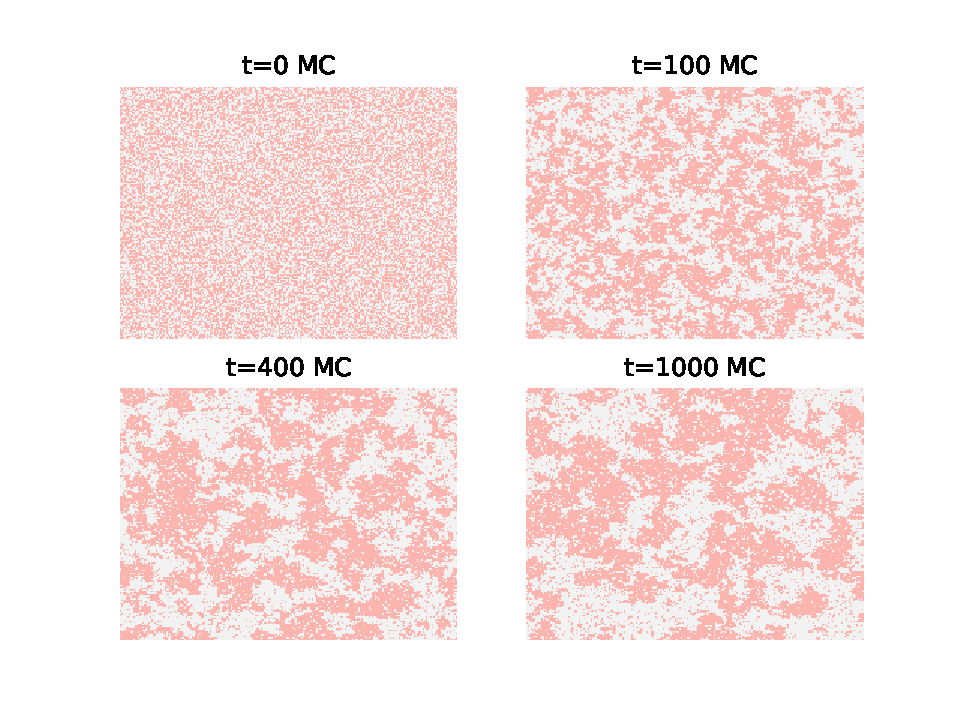
\includegraphics[width=0.9\linewidth]{intro/clusterization.pdf}
    \caption{Phénomène d'aggrégation à partir d'une trempe (\textit{quench}) dans un modèle d'Ising de $T=\infty$ à $T=T_{2D,C}$ \cite{onsager_crystal_1944} pour différents temps en étapes de Monte Carlo, pour un système $600 \times 600$ avec une dynamique non-conservée de Glauber.}
    \label{clusterization}
\end{figure}


In this chapter we will analyse the dynamics of statistical systems. The analysis will allow us to understand how phase transitions occur dynamically. For instance we know that certain systems undergo what is known phase separation, for instance if we take the Ising model with zero magnetic field, in the high temperature phase the system is homogeneous and the average magnetisation, which is the order parameter for the transition is zero. Below the critical temperature if the overall magnetisation is conserved (for instance for Kawasaki dynamics), which would be the case if spins corresponded to different types of particles, the system will separate into two  phases of opposite average magnetisation, separated by an interface which will be roughly flat in order to minimise the surface energy between the two phases. For nonconserved systems, where the overall magnetisation in not conserved (for example Glauber dynamics), eventually one of the two phases will make up the system (spontaneous symmetry breaking). In a continuous phase transition as the critical point is reached from the disordered to ordered, domains of phases of positive and negative magnetisation form and the size of these domains is given by the correlation length of the system. For continuous phase transitions such as that in the Ising model the correlation length diverges as as the critical point is approached, for instance as $T\to T_c$ if the temperature is varied. The size of the domains thus have to become infinite if the system is infinite, this means that for an infinite system it will take an infinite time to relax to the equilibrium state. The process of domain growth is known as coarsening and phase ordering kinetics is the theory that has been developed to understand the phenomenon of coarsening. Furthermore, for systems with a conserved order parameter which separate into two phases, the two phases will be separated by an interface. This interface will be characterised by a surface tension, its average position will be fixed but it will exhibit fluctuations. Later we will see how model of phase ordering kinetics and be used to determine the static and dynamical properties of interfaces between two coexisiting phases. 

While the phase diagram of a system can be determined via 
its Hamiltonian and equilibrium statistical mechanics, the dynamics of coarsening depends on details of the systems dynamics that do not show up in single time thermodynamic observables. Therefore one needs to construct dynamical models that capture the underlying evolution of the state of the system, in particular there is a big difference between systems where the order parameter is conserved and those where it is not conserved.

\section{Statics of systems with a finite number of degrees of freedom}

Thermodynamic systems are naturally described in terms of fields, for example densities. This means that one is naturally lead to consider statistical field theories where the system is described in terms of a local field $\phi({\bf x})$. Statistical field theories can be applied to both statics, to understand phase diagrams, and dynamics to understand phase ordering. However to start with we will examine the case of systems with a finite number of degrees of freedom. 

Consider a system in the canonical ensemble with a Hamiltonian $H({\bf q})$ where $q_i$ for 
$1\leq i\leq N$ represent a finite number of continuous spatial degrees of freedom and where in a classical system we have already integrated over the corresponding momenta. The partition function for the system is given by
\begin{equation}
Z = \int d{\bf q} \exp\left(-\beta H({\bf q})\right),
\end{equation}
and in equilibrium the probability density function $P_{eq}({\bf q})$ of the degrees of freedom is given by 
\begin{equation}
P_{eq}({\bf q}) = \frac{\exp\left(-\beta H({\bf q})\right)}{Z}.\label{eqdis}
\end{equation}
In general the integral which gives the  partition function cannot be computed analytically.
The simplest approximation to compute $Z$ is the mean field approximation where the integral 
is approximated by the integrand at its largest value - in mathematics this is the Laplace method for approximating an integral and in this context it is just an expansion about the minimum energy configuration of the system. The mean field approximation is thus
\begin{equation}
Z_{MF}= \exp\left(-\beta H({\bf q}^*)\right),
\end{equation}
where ${\bf q}^*$ is the value of ${\bf q}$ which minimises $H$ (note that the approximation becomes exact in the zero temperature limit - $\beta \to \infty$   - as the system will minimise its energy). The values $q_i^*$ are determined from
\begin{equation}
\frac{\partial H}{\partial q_i}|_{{\bf q}={\bf q^*}}=0.
\end{equation}
Within this approximation any thermodynamic observable is given by
\begin{equation}
\langle f({\bf q}) \rangle = f({\bf q}^*).
\end{equation}

We now consider how one can model dynamics of such systems. We will look for a Langevin equation which is chosen to give the correct equilibrium Gibbs-Boltzmann distribution. We write
\begin{equation}
\frac{d q_i}{dt} = -L_{ij}\frac{\partial H({\bf q})}{ \partial q_j} + \eta_i(t),
\end{equation}
where $L_{ij}$ is a matrix which discuss later and $\eta_i(t)$ is zero mean Gaussian white noise  with correlation function 
\begin{equation}
\langle \eta_i(t)\eta_j(t')\rangle =  \Gamma_{ij} \delta(t-t')\label{cfn}
\end{equation}
The Gaussian white noise represents the effects of thermal fluctuations on the system we assume that the correlation time of these fluctuations is extremely short with respect to the dynamics of the degrees of freedom $q_i$ (in fact in critical systems the dynamics becomes very slow, critical slowing down, and this approximation becomes better and better as one approaches the critical point).  There is no momentum term in this Langevin equation and for this reason it is often called the over damped Langevin equation. Overdamped Langevin equations can also be derived staring from Newton's laws in the presence of friction, due to a solvent, and again white noise (again due to molecular collisions with the solvent) and by taking the limit where the frictional forces are greater than the acceleration term in Newton's equations (equivalent to setting the particle masses to zero).


As Eq. (\ref{cfn}) is for a correlation function the matrix $\Gamma_{ij}$ must be symmetric and cannot have any negative eigenvalues.

In the absence of noise or thermal fluctuations, so at zero temperature, the system will simply minimise its energy. Therefore if 
\begin{equation}
\frac{\partial H({\bf q})}{ \partial q_j} =0, 
\end{equation}
with no noise we have $\frac{d q_i}{dt}=0$, that is to say it is the term $\frac{\partial H({\bf q})}{ \partial q_j}$ that drives the dynamics if there is no noise. As long as the matrix $L_{ij}^{-1}$ exists the zero temperature dynamics will take the system to the local minimum of $H$ and to the absolute minimum if there are no metastable configurations. 

Under these assumptions, the Fokker-Planck equation for the probability density function of the degrees of freedom is 
\begin{equation}
\frac{\partial p({\bf q},t)}{\partial t} = \frac{\partial}{\partial q_i} \left[\frac{1}{2}\Gamma_{ij} \frac{\partial p({\bf q},t)}{\partial q_i} + p({\bf q},t) L_{ij}\frac{\partial H({\bf q})}{ \partial q_j}\right].
\end{equation}
This can be written as 
\begin{equation}
\frac{\partial p({\bf q},t)}{\partial t} +\frac{\partial}{\partial q_i}J_i({\bf q},t)=0,
\end{equation}
where the ${\bf J}({\bf q},t)$ is the probability current. We now insist that the system is in equilibrium with zero current when $p({\bf q},t)= P_{eq}({\bf q})$ as given by Eq. (\ref{eqdis}), this gives
\begin{equation}
\left[-\frac{\beta}{2}\Gamma_{ij} + L_{ij}\right]\frac{\partial H({\bf q})}{ \partial q_j},
\end{equation}
and this holds for any choice of $H$ is we chose.
\begin{equation}
\Gamma_{ij}= 2T L_{ij}
\end{equation}
where we have taken units where Boltzmann's constant $k_B=1$. 
\section{Statistical field theory}
We now consider a system with Hamiltonian $H[\phi]$ which depends on a continuous field 
$\phi({\bf x})$. The partition function is given by a functional integral
\begin{equation}
Z = \int d[\phi] \exp(-\beta H[\phi]),
\end{equation}
the functional integral over all possible fields $\phi$ can be taken as a limit where $\phi$ is defined at a finite number of points on a lattice and then the lattice spacing is taken to zero. 
In many cases  the system has been coarse grained and $\phi$ represents a spatially varying order parameter, for instance the local density averaged over some small volume. In this case the Hamiltonian $H$ is strictly speaking a free energy  and contains terms that depend on the temperature.

The mean field approximation to partition function is then given by
\begin{equation}
Z _{MF}=  \exp(-\beta H[\phi_{MF}]),
\end{equation} 
where $\phi_{MF}$ is the mean field solution which minimises $H$. The definition of a functional derivative of a functional is
\begin{equation}
F[\phi+\delta\phi]-F[\phi]= \int d{\bf x} \frac{\delta F}{\delta\phi({\bf x})} \delta\phi({\bf x}).
\end{equation}
Therefore if a field $\phi$ maximises $H$ we must have 
\begin{equation}
\frac{\delta H}{\delta\phi({\bf x})}=0.
\end{equation}

We now consider the standard Landau-Ginzburg Hamiltonian describing Ising like systems where
\begin{equation}
H[\phi] = \int d{\bf x} \ \frac{\kappa}{2}[\nabla \phi]^2 + V(\phi) .
\end{equation}
The first term represents an energetic cost of varying the field $\phi$ while the second potential term has two minima at $\phi=\pm \phi_c$, and without loss of generality we can chose  $V(\phi_c)=V(-\phi_c)$, in the low temperature or phase separated phase and a single minimum at $\phi=0$ in the high temperature phase. The standard, so called, $\phi^4$ form is
\begin{equation}
V(\phi) = \frac{1}{2} m^2 \phi^2 + \frac{\lambda}{4!} \phi^4,\label{p4}
\end{equation} 
where 
\begin{equation}
m^2 = T-T_c.
\end{equation}
It is easy to see that 
\begin{equation}
\frac{\delta H}{\delta \phi({\bf x})} = -\kappa \nabla^2 \phi({\bf x}) + V'(\phi).\label{cm}
\end{equation}
If there is non constraint on the system if can simply chose $\phi({\bf x}) =\phi_c$ or $\phi({\bf x}) =-\phi_c$ everywhere which corresponds to a  free energy $F=H[\phi_c]=0$. However in a system with a conserved order parameter
\begin{equation}
\int d{\bf x} \  \phi({\bf x})=0, 
\end{equation}
then the solutions $\phi=\pm \phi_c$ cannot hold. In this case the system will separate into a two phases where $\phi({\bf x})= \pm \phi_c$. We therefore choose an interface at $z=0$ where 
and take $\phi({\bf x}) = \phi_K(z)$ ($K$ standing for kink as it is known as the kink solution in the literature) where $\lim_{z\to\-\infty}=-\phi_c$ and  $\lim_{z\to\infty}=-\phi_c$. 
We therefore find from Eq. (\ref{cm}) that
\begin{equation}
-\kappa \frac{d^2 }{dz^2}\phi_K(z)  + V'(\phi_K) = 0 \label{kk0}
\end{equation}
This equation can be solved for the potential in \eqref{p4} ({\em you should do it and fill in the details}) but even without knowing the explicit solution we can write
\begin{equation}
H[\phi_K]=  A\int dz \ \frac{\kappa}{2}\left(\frac{d\phi_K(z)}{dz}\right)^2 + V(\phi_K(z)),\label{kk1}
\end{equation}
where $A$ is the surface area of the system in the plane perpendicular to the direction $z$. 
However if we multiply Eq. \eqref{kk0} by $d\phi/dz$ and integrate we find
\begin{equation}
-\frac{\kappa}{2} (\frac{d\phi_K}{dz})^2 + V(\phi_K) = C,
\end{equation}
where $C$ is a constant. However as $\phi_K(z)\to \pm \phi_c$ as $z\to \pm \infty$ and $V(\pm\phi_c) =0$ we find that $C=0$. Using this we obtain 
\begin{equation}
H[\phi_K]=  A\int dz\  {\kappa}\left(\frac{d\phi_K(z)}{dz}\right)^2 .
\end{equation}
If the interface has a free energy per unit area of $\sigma$ then we have the Cahn-Hillard estimate of the surface tension 
\begin{equation}
\sigma=  \int dz\  {\kappa}\left(\frac{d\phi_K(z)}{dz}\right)^2 .\label{CHST}
\end{equation}

Now we return to dynamics. If we compare with systems with a discrete number of variables we
should have a Langevin equation of the form
\begin{equation}
\frac{\partial \phi({\bf x})}{\partial t}= -L \frac{\delta H}{\delta \phi({\bf x})} + \eta({\bf x},t).
\end{equation}
The white noise correlator should have the form
\begin{equation}
\langle \eta({\bf x},t)\eta({\bf x}',t)\rangle =\delta(t-t')\Gamma({\bf x},{\bf x'}),
\end{equation}
where here  $\Gamma({\bf x},{\bf x'})$ is an operator (before it was a matrix) defined by its action on functions $f$ as
\begin{equation}
\Gamma f({\bf x}) = \int d{\bf x}' \Gamma({\bf x},{\bf x}')f({\bf x}'),
\end{equation}
and $L$ is also an operator with 
\begin{equation}
L f({\bf x}) = \int d{\bf x}' L({\bf x},{\bf x}')f({\bf x}'),
\end{equation}
Following the same arguments for systems with a finite number of degrees of freedom we thus have the relation (which is sometimes called the fluctuation dissipation theorem as it essentially is equivalent)
\begin{equation} 
\Gamma({\bf x},{\bf x}') =2T L({\bf x},{\bf x}').\label{gnoise}
\end{equation}
The simplest form of dynamics is given by $L({\bf x},{\bf x}')=\alpha\delta({\bf x}-{\bf x}')$ which gives the model A dynamics
\begin{equation}
\frac{\partial \phi({\bf x})}{\partial t}= -\alpha \frac{\delta H}{\delta \phi({\bf x})} + \eta({\bf x},t),\label{MA}
\end{equation}
with the noise correlator
\begin{equation}
\langle \eta({\bf x},t)\eta({\bf x}',t)\rangle =2T \alpha \delta(t-t')\delta({\bf x}-{\bf x'}).
\end{equation}
The average value of $\phi$ 
\begin{equation}
\overline \phi(t) = \frac{1}{V}\int d{\bf x}\  \phi({\bf x},t),
\end{equation}
is clearly not generally conserved by this dynamics.

Model $B$ dynamics amounts to choosing
\begin{equation}
L({\bf x}-{\bf x}')= -D\nabla^2 \delta({\bf x}-{\bf x'}),
\end{equation}
here the fact that $L$ is a positive semi-definite operator can be seen by taking its Fourier transform. The evolution equation here is
\begin{equation}
\frac{\partial \phi({\bf x})}{\partial t}= D\nabla^2 \frac{\delta H}{\delta \phi({\bf x})} + \eta({\bf x},t),
\label{MB}
\end{equation}
and where
\begin{equation}
\langle \eta({\bf x},t)\eta({\bf x}',t)\rangle =-2TD   \delta(t-t')\nabla^2\delta({\bf x}-{\bf x'}).
\end{equation}
We notice that if we introduce the vectorial white noise with components $\eta_i({\bf x},t)$ such that
\begin{equation}
\langle \eta_i({\bf x},t) \eta_i({\bf x}',t')\rangle =\delta_{ij} \delta({\bf x}-{\bf x'})\delta(t-t),
\end{equation}
where $\delta_{ij}=1$ for $i=j$ and is zero otherwise,  we can write
\begin{equation}
\eta({\bf x},t)= \nabla\cdot {\boldsymbol \eta}({\bf x},t),
\end{equation}
as one can verify the two noises have the same correlation function. In this way Eq. (\ref{MB}) becomes 
\begin{equation}
\frac{\partial \phi({\bf x})}{\partial t}= \nabla\cdot[ D\nabla \frac{\delta H}{\delta \phi({\bf x})} + {\boldsymbol\eta}({\bf x},t)].
\end{equation}
From this it is easy to see that the order parameter is conserved - thus model  B describes conserved phase ordering dynamics.

\section{Models for equilibrium interfaces}
Here we discuss effective models of interfaces. The simplest model is to assume that the 
interface is parameterised by a height profile $h({\bf r})$, however one also has to assume that 
$h({\bf r})$ is a single valued function of ${\bf r}$. Given this one can write
\begin{equation}
H[h] = \sigma A[h]
\end{equation}
where $A_h$ is the area of the interface. However the interface area is given by
\begin{equation}
A[h] = \int_A d{\bf r}\sqrt{1+[\nabla h]^2},
\end{equation}
where the integral is over the plane perpendicular to the $z$ axis which is taken to be of area $A$. When the fluctuations of the interface are small, we can expand the above to quadratic order in $h$ to obtain
\begin{equation}
H[h]= A\sigma +\frac{\sigma}{2} \int_A d{\bf r} \ [\nabla h]^2.
\end{equation}
The first term is independent of the height so we can write the effective Hamiltonian for the surface as
\begin{equation}
H_{eff} [h]= \frac{\sigma}{2} \int_A d{\bf r}\  [\nabla h]^2.\label{heff}
\end{equation}
\section{Effective dynamics of interface heights}\label{heightd}
We will now try and derive an approximation for the dynamics of the  height of the interface from the original phase ordering kinetics. Here we use the method of Bray and Cavagnha - put in the reference, which was used to study the dynamics of sheared interfaces, in the absence of shear to determine the dynamical properties of interfaces in phase separated systems for both model A and model B dynamics.

We imagine that the system is phase separated in the direction  $z$, on average the interface is taken to be at $z=0$, and we write
\begin{equation}
\phi(z,{\bf r},t) = f(z-h({\bf r},t))\label{hans}
\end{equation}
where $f(z)=\phi_K(z)$ is the kink solution from mean field theory.
\\

\noindent{\bf Model A dynamics}

For model A dynamics, we substitute Eq. \eqref{hans} into Eq. \eqref{MA} and make use of the following results
\begin{eqnarray}
\frac{\partial f(z-h({\bf r},t))}{\partial t}&=& -f'(z-h({\bf r},t))\frac{\partial h({\bf r},t)}{\partial t}\\
\nabla f(z-h({\bf r},t))&=& [{\bf e}_z-\nabla h({\bf r},t)]f'(z-h({\bf r},t))  \\
\nabla^2 f(z-h({\bf r},t))&=& f''(z-h({\bf r},t))- \nabla^2 h({\bf r},t)f'(z-h({\bf r},t))+ [\nabla h({\bf r},t)]^2 
f''(z-h({\bf r},t))
\end{eqnarray}
and thus find
\begin{eqnarray}
&&-f'(z-h({\bf r},t))\frac{\partial h({\bf r},t)}{\partial t}= \alpha\kappa\times\\ &&\left[f''(z-h({\bf r},t))- \nabla^2 h({\bf r},t)f'(z-h({\bf r},t))+ [\nabla h({\bf r},t)]^2 
f''(z-h({\bf r},t))\right] - \alpha V'(f'(z-h({\bf r},t))) + \eta({\bf r},z,t).
\end{eqnarray}
We now multiply both sides of this equation by $f'(z-h({\bf r},t))$ and defining $\zeta=z-h({\bf r},t)$ we integrate  $\zeta$ over $[-\infty,\infty]$ and use the following identities
\begin{eqnarray}
\int_{-\infty}^\infty d\zeta f'(\zeta)f''(\zeta) &=& [\frac{1}{2}f'^2(\zeta)]_{-\infty}^\infty =0\\
\int_{-\infty}^\infty d\zeta f'(\zeta) V'(f) &=& \int_{-\infty}^\infty d\zeta\frac{d V(f)}{d\zeta}= [V(f(\zeta))]_{-\infty}^\infty=0,
\end{eqnarray} 
note that the first relation above holds as $f(\zeta)=\pm \phi_c$ as $\zeta\to\pm \infty$ and the second as
$V(\phi_c)=V(-\phi_c)=0$.
The terms that are left then give
\begin{equation}
-\int_{-\infty}^\infty f'^2(\zeta)d\zeta\ \frac{\partial h({\bf r},t)}{\partial t}
= -\alpha\int_{-\infty}^\infty f'^2(\zeta)d\zeta \ \kappa \nabla^2 h({\bf r},t) + \int_{-\infty}^\infty d\zeta \eta({\bf r},\zeta+ h({\bf r},t))f'(\zeta)
\end{equation}
Now using the Cahn-Hillard estimate of the surface tension Eq. \eqref{CHST} this becomes
\begin{equation}
\frac{\sigma}{\kappa} \frac{\partial h({\bf r},t)}{\partial t}
= \alpha\sigma \nabla^2 h({\bf r},t) +\xi({\bf r},t),
\end{equation}
where the noise term is given by
\begin{equation}
\xi({\bf r},t)= \int_{-\infty}^\infty d\zeta \eta({\bf r},\zeta+ h({\bf r},t))f'(\zeta)
\end{equation}
The noise term has zero mean and correlation function
\begin{eqnarray}
\langle \xi({\bf r},t)\xi({\bf r}',t')\rangle &=&2\alpha T\delta(t-t')\delta({\bf r}-{\bf r}')\int_{-\infty}^\infty d\zeta d\zeta' \delta(\zeta-\zeta')f'(\zeta)f'(\zeta')\\
&=& 2\alpha T\delta(t-t')\delta({\bf r}-{\bf r}')\int_{-\infty}^\infty d\zeta f'^2(\zeta)= \frac{2\alpha T\sigma}{\kappa}\delta(t-t')\delta({\bf r}-{\bf r}').
\end{eqnarray}
This now gives
\begin{equation}
\frac{\partial h({\bf r},t)}{\partial t}= \kappa\alpha \nabla^2 h({\bf r},t) + \eta({\bf r},t)
\end{equation}
where 
\begin{equation}
\langle \eta({\bf r},t)\eta({\bf r}',t')\rangle = \frac{2\alpha T\kappa}{\sigma}\delta(t-t')\delta({\bf r}-{\bf r}').
\end{equation}
Now defining $\alpha' = \frac{\kappa\alpha}{\sigma}$ we can write
\begin{equation}
\frac{\partial h({\bf r},t)}{\partial t}= \alpha' \sigma\nabla^2 h({\bf r},t) + \eta({\bf r},t).
\end{equation}
This has the form of model $A$ dynamics (as in Eq. \eqref{MA})  for the height profile with Hamiltonian
$H_{eff}$ as given in \eqref{heff}, that is to say we can write
\begin{equation}
\frac{\partial h({\bf r},t)}{\partial t}= -\alpha' \frac{\delta H_{eff}[h]}{\delta h({\bf r})} + \eta({\bf r},t),
\label{ew}
\end{equation}
and where 
\begin{equation}
\langle \eta({\bf r},t)\eta({\bf r}',t')\rangle= 2T\alpha'\delta(t-t').
\end{equation}
This dynamical calculation is thus consistent with the idea of describing the surface in terms of a height variable with an energy given by the surface tension. The equation \eqref{ew} is known as the Edwards-Wilkinson equation. We can use this equation to determine how the domains of a coarsening systems grow at low temperatures. To do this we ignore the noise term and assume that at $t=0$ the correlations of the height are short range so
\begin{equation}
C({\bf r}-{\bf r}',0)= \langle h({\bf r},0)h({\bf r}',0)\rangle =C_0 \delta({\bf r}-{\bf r}').
\end{equation}
In Fourier space the noiseless Edwards-Wilkinson equation becomes
\begin{equation}
\frac{\partial\tilde h({\bf k},t)}{\partial t} = -\alpha'\sigma \tilde h({\bf k},t) ,
\end{equation}
and so we find
\begin{equation}
\tilde h({\bf k},t) = h({\bf k},0)\exp(-\alpha'\sigma{\bf k}^2 t).
\end{equation}
We thus find 
\begin{equation}
\langle \tilde h({\bf k},t)\tilde h({\bf k}',t')\rangle = \langle h({\bf k},0)h({\bf k}',0)\rangle \exp(-\alpha'\sigma[k^2+k'^2] t).
\end{equation}
Now recall that if 
\begin{equation}
\langle  h({\bf r},t) h({\bf r}',t')\rangle =C({\bf r}-{\bf r}',t)
\end{equation}
then
\begin{equation}
\langle \tilde h({\bf k},t)\tilde h({\bf k}',t')\rangle= (2\pi)^d \delta({\bf k}+{\bf k}') \tilde C({\bf k},t),
\end{equation}
where 
\begin{equation}
\tilde C({\bf k},t)= \int d{\bf r} \exp(-i{\bf k}\cdot {\bf r})C({\bf r},t),
\end{equation}
is the Fourier transform of the correlation function which is a function of a single position due to invariance by translation in space, and $d$ is the dimension of space (so here $d=2$ for a surface in 3d space and $d=1$ for a surface in a 2d space). Putting all this together gives
\begin{equation}
\tilde C({\bf k},t)= C_0 \exp(-2\alpha'\sigma k^2 t).
\end{equation}
Inverting the Fourier transform gives
\begin{equation}
C({\bf r},t)= \frac{C_0}{(8\pi \alpha'\sigma t)^{\frac{d}{2}}} \exp(-\frac{{\bf r}^2}{16\pi \alpha'\sigma t}).
\end{equation}
From this we see that if $C({\bf r},t)\sim g(\frac{{\bf r}}{\ell(t)})r(t)$ then the length scale $\ell(t)\sim t^{\frac{1}{2}}$, this agrees with is found in the Ising model under Glauber dynamics, where the growth exponent is also given by $z=\frac{1}{2}$.
\\

\noindent{\bf Model B dynamics}

For model B dynamics, we take the same ansatz as in Eq. \eqref{hans} but we rewrite the model B dynamics as
\begin{equation}
-\nabla^{-2} \frac{\partial\phi({\bf x},t)}{\partial t} = -D \frac{\delta H}{\delta \phi({\bf x})}+ 
\theta({\bf x},t),
\end{equation}
here $-\nabla^{-2}$ represents the Green's function $G$ which obeys 
\begin{equation}
\nabla^2 G({\bf x}-{\bf x'}) = -\delta({\bf x}-{\bf x}'),
\end{equation}
and 
\begin{equation}
\theta({\bf x},t)=-\nabla^{-2}\eta({\bf x},t)= \int d{\bf x}'G({\bf x}-{\bf x'})\eta({\bf x},t)
\end{equation}
The correlation function of $\theta({\bf x},t)$ is given by
\begin{eqnarray}
\langle \theta({\bf x},t)\theta({\bf y},t')\rangle &=&-2DT\delta(t-t') \int d{\bf x}'G({\bf x}-{\bf x'})d{\bf y}'G({\bf y}-{\bf y'})\nabla^2\delta({\bf x}'-{\bf y}') \\
&=& -2DT\delta(t-t') \int d{\bf x}'G({\bf x}-{\bf x'})d{\bf y}'\nabla^2G({\bf y}-{\bf y'})\delta({\bf x}'-{\bf y}') \\
&=& 2DT\delta(t-t') G({\bf x}-{\bf y}).
\end{eqnarray}
where we have integrated by parts in the second line and used 
\begin{equation}
-\nabla^2G({\bf y}-{\bf y'})= \delta({\bf y}-{\bf y}'),
\end{equation}
in the third.

Now mutliplying by $f'(z-h({\bf r},t))$ and integrating $z$ over $[-\infty,\infty]$, we find
\begin{eqnarray}
&&-\int dz f'(z-h({\bf r},t))\int dz'd{\bf r}'\  G(z-z',{\bf r}-{\bf r}') f'(z'-h({\bf r}',t))\frac{\partial h({\bf r}',t)}{\partial t} = \\
&&-D\sigma \nabla^2 h({\bf r},t) + \chi({\bf r},t),
\end{eqnarray}
with the noise
\begin{equation}
\chi({\bf r},t)= \int dz f'(z-h({\bf r},t)) \theta({\bf r},z,t).
\end{equation}
As we assume that the height fluctuations are small we keep only the lowest order terms in $h$ in the deterministic terms and the noise, we will see later that this is compatible thermodynamically. We thus have
\begin{eqnarray}
&&-\int dz \ f'(z)\int dz'd{\bf r}'\  G(z-z',{\bf r}-{\bf r}') f'(z')\frac{\partial h({\bf r}',t)}{\partial t} = \\
&&-D\sigma \nabla^2 h({\bf r},t) + \chi({\bf r},t),
\end{eqnarray}
and now  the noise is given by
\begin{equation}
\chi({\bf r},t)= \int dz\  f'(z) \theta({\bf r},z',t).
\end{equation}
This equation which is linear in $h$ can now be Fourier transformed in the plane ${\bf r}$ and in terms of the Fourier transform of $h$ we find
\begin{equation}
-\int dz \ f'(z)\int dz'd{\bf r}'\ \tilde G(z-z',{\bf k}) f'(z')\frac{\partial\tilde h({\bf k},t)}{\partial t} = 
Dk^2\sigma \tilde h({\bf k},t) + \tilde \chi({\bf k},t).\label{bstep}
\end{equation}
The Fourier transform of $G$ in the ${\bf r}$ plane obeys
\begin{equation}
\frac{d^2 \tilde G(z-z',{\bf k} )}{dz^2}-k^2 \tilde G(z-z',{\bf k} )=-\delta(z-z')
\end{equation}
and the solution to this equation (with the boundary condition that $\tilde G(z-z',{\bf k} )\to 0$ as $|z-z'|\to\infty$)  is
\begin{equation}
\tilde G(z-z',{\bf k}) = \frac{\exp(-k|z-z'|)}{2k},
\end{equation}
and note that $k=|{\bf k}|$. 
Next we make the sharp interface approximation where we write
\begin{equation}
f(z) = 2\phi_c \delta(z),\label{sharp}
\end{equation}
that is to say we have replaced the smooth kink solution with a step like solution
$f(z) = \phi_c\  {\rm sgn}(z)$. This then gives
\begin{equation}
-4\phi_c^2 \tilde G(0,k) \frac{\partial h({\bf k},t)}{\partial t} = 
Dk^2\sigma  \tilde h({\bf k},t) + \tilde \chi({\bf k},t),
\end{equation}
which we rewrite as
\begin{equation}
\frac{\partial \tilde h({\bf k},t)}{\partial t} = -\frac{Dk^3\sigma}{2\phi_c^2} \tilde h({\bf k},t) + \tilde \xi({\bf k},t),
\end{equation}
with 
\begin{equation}
\tilde \xi({\bf k},t)= - \frac{k}{2\phi_c^2}\tilde \chi({\bf k},t),
\end{equation}
where 
\begin{equation}
\tilde \chi({\bf k},t)= \int dz\  f'(z) \tilde\theta({\bf k},z,t),
\end{equation}
The correlation function of $\tilde \theta({\bf k},t)$ is 
\begin{equation}
\langle \theta({\bf k},t)\theta({\bf k}',t')\rangle = 2DT(2\pi)^d \delta(t-t') \delta({\bf k}+{\bf k'}) \tilde G(z-z',k)
\end{equation}
and from this we find 
\begin{equation}
\langle \chi({\bf k},t)\chi({\bf k}',t')\rangle  = 2DT(2\pi)^d \delta(t-t') \delta({\bf k}+{\bf k'}) \int dz dz'
f(z) f(z') \tilde G(z-z',k),\label{bstep2}
\end{equation}
now using the sharp interface approximation Eq. (\ref{sharp}) we obtain
\begin{equation}
\langle \chi({\bf k},t)\chi({\bf k}',t')\rangle  = 2DT(2\pi)^d \delta(t-t') \delta({\bf k}+{\bf k'}) \frac{2\phi_c^2}{k},
\end{equation}
and consequently
\begin{equation}
\langle \xi({\bf k},t)\xi({\bf k}',t')\rangle = 2DT(2\pi)^d \delta(t-t') \delta({\bf k}+{\bf k'}) \frac{k}{2\phi_c^2}.
\end{equation}
Finally in we find the interface dynamics for model B in Fourier space is
\begin{equation}
\frac{\partial h({\bf k},t)}{\partial t} = -\frac{Dk^3\sigma}{2\phi_c^2} \tilde h({\bf k},t) + \tilde \xi({\bf k},t),\label{modBFT}
\end{equation}
In real space this has the form
\begin{equation}
\frac{\partial h({\bf r})}{\partial t}= -L \frac{\delta H_{eff}}{\delta h ({\bf r})} + \xi({\bf r},t).
\end{equation}
where the operator $L$ is defined via its Fourier transform
\begin{equation}
\tilde L({\bf k}) = \frac{Dk}{2\phi_c^2}.
\end{equation}
Now if we look at Eq. \eqref{modBFT} we see that solving the equation without noise will give a function of $k^3t$, which in real space corresponds to $x^3/t$. From this we see that the coarsening length scale grows as $\ell(t) \sim t^{\frac{1}{3}}$ and consequently the coarsening exponent is $z=\frac{1}{3}$.  Coarsening for conserved model B or diffusive dynamics is slower than that of model A. One of the reasons for this slowing down with respect to nonconserved dynamics is that material must be physically transported by diffusion (by exchanging spins in the language of lattice spin models), where as for  model A dynamics the composition can change at any given point by {\em spin flipping}. As a cautionary note, if we had taken the
Hamiltonian in Eq. \eqref{heff} and applied model B conserved dynamics, as in Eq. \eqref{MB},  for the height field we would not have obtained this equation. 

We can actually do better than the above sharp interface approximation as Eq. \eqref{bstep} can be written as
\begin{equation}
Q(k)\frac{\partial\tilde h({\bf k},t)}{\partial t} = 
-Dk^2\sigma \tilde h({\bf k},t) - \tilde \chi({\bf k},t).\label{bstep2}
\end{equation}
where 
\begin{equation}
Q(k)= \int dzdz' \ f'(z)\ \tilde G(z-z',{\bf k}) f'(z').
\end{equation}
Notice that from Eq. \eqref{bstep2} that
\begin{equation}
\langle \chi({\bf k},t)\chi({\bf k}',t')\rangle  = 2DT(2\pi)^d \delta(t-t') \delta({\bf k}+{\bf k'}) Q(k).\end{equation}
and so 
\begin{equation}
\frac{\partial\tilde h({\bf k},t)}{\partial t}= -\tilde L(k) \tilde \mu({\bf k}) + \eta({\bf k}),
\end{equation}
where $\mu({\bf x})=\delta H_{eff}/\delta h({\bf x}) $ and $\tilde L(k) = D/Q(k)$ and 
\begin{equation}
\langle \eta({\bf k},t)\eta({\bf k}',t')\rangle  = 2T(2\pi)^d \delta(t-t') \delta({\bf k}+{\bf k'}) \tilde L(k).\end{equation}
\section{Systems driven by imposed hydrodynamic flows}
{\bf Here you need to discuss the experiments get some nice photos etc}

Here we consider what happens when a system is driven out of equilibrium, by driven we mean that energy is injected into the system by a laser for instance as discussed in the introduction or by inducing a hydrodynamics flow, for instance a shear flow induced in a Couette cell. In principle we should analyse this system with model H dynamics which couples diffusive model B dynamics to hydrodynamics in the low Reynolds number Stokes flow regime. In this dynamics the order parameter field will itself induce a hydrodynamics flow which will modify
the imposed one. However this full situation is very difficult to analyse and to a first approximation we can assume that the back reaction of the order parameter field on the hydrodynamic flow is small with respect to the imposed hydrodynamic flow and so we can simply write
\begin{equation}
\frac{\partial \phi ({\bf x},t)}{\partial t} + \nabla\cdot({\bf  v}({\bf x})\phi({\bf x},t)) =- L\frac{\delta H}{\delta \phi({\bf x})} + \eta({\bf x},t),\label{drive}
\end{equation}
where $L$ is given by the underlying model A or B dynamical operatorand the noise has the correlation function as given by Eq. \eqref{gnoise}, and ${\bf v}({\bf x})$ is the imposed (time independent) hydrodynamic flow or can equally well be an external drive imposed on the colloidal particles, due to the gravitational or electric field for example. 

The simplest case one can consider is where the driving field ${\bf v}({\bf x}) ={\bf v}_0$ is uniform . Unfortunately this simple driving does not lead to a new steady state. Basically all of the colloidal particles acquire an an average velocity ${\bf v}$ and so move along at the same speed relative to each other. Mathematically this can be seen by making the Galilean transformation
\begin{equation}
\phi ({\bf x},t)= \phi({\bf x}-{\bf v}_0t,t) = \phi({\bf y},t).
\end{equation}
this transform eliminates the driving from the evolution equation \eqref{drive} and so we find an equilibrium system. 

The most studies example is where the driving is a shear flow, this corresponds to the experiments of Derks et al and the numerical simulations of Smith et al and the analytical work
of Bray and Cavagnah. In Bray and Cavagna, the effective dynamics of the surface term 
in the presence of a shear flow, parallel to the interface,
\begin{equation}
{\bf v}({\bf x}) = \gamma z {\bf e}_x
\end{equation}
was studied using the method explained in section (\ref{heightd}). The addition of a shear flow leads to the appearance of a nonlinear term in $h$ and the interface statistics thus become non-Gaussian.

